% Gemini theme
% See: https://rev.cs.uchicago.edu/k4rtik/gemini-uccs
% A fork of https://github.com/anishathalye/gemini

\documentclass[final]{beamer}

% ====================
% Packages
% ====================

\usepackage[T1]{fontenc}
\usepackage{lmodern}
\usepackage[size=custom,width=48in,height=36in,scale=1.0]{beamerposter}
\usetheme{gemini}
\usecolortheme{uchicago}
\usepackage{graphicx}
\usepackage{subfig}
\usepackage{booktabs}
\usepackage{tikz}
\usepackage{pgfplots}
\usepackage{multicol}
\pgfplotsset{compat=1.17}

% ====================
% Lengths
% ====================

% If you have N columns, choose \sepwidth and \colwidth such that
% (N+1)*\sepwidth + N*\colwidth = \paperwidth
\newlength{\sepwidth}
\newlength{\colwidth}
\setlength{\sepwidth}{0.025\paperwidth}
\setlength{\colwidth}{0.3\paperwidth}

\newcommand{\separatorcolumn}{\begin{column}{\sepwidth}\end{column}}

% ====================
% Title
% ====================

\title{The Effects of Affordable Housing on New York City Public Health \protect\\ 
Mitigating the COVID-19 Pandemic through Housing}

\author{Andrew G. Argeros \& Elias A. Ramirez}

\institute[shortinst]{Hamline University School of Business}



% ====================
% Footer (optional)
% ====================

\footercontent{
  \href{https://www.hamline.edu}{www.hamline.edu} \hfill
  BAC @ MC 2021 -- Virtual \hfill
  \href{mailto:aargeros01@hamline.edu}{aargeros01@hamline.edu}}
% (can be left out to remove footer)

% ====================
% Logo (optional)
% ====================

% use this to include logos on the left and/or right side of the header:
\logoright{
\includegraphics[height=9cm]{pics/Hamline_HSB_stacked_white.png}}
\logoleft{
\includegraphics[height=9cm]{pics/HU sep shield red.png}}

% ====================
% Body
% ====================

\begin{document}
% \addtobeamertemplate{headline}{}
% {
%     %\begin{tikzpicture}[remember picture,overlay]
%       %\node [anchor=north west, inner sep=3cm] at ([xshift=-1cm,yshift=-2.75cm]current page.north west)
%      % {\includegraphics[height=5.0cm]{logos/SHS+Excelera_logo_white (1).png}};
%     %\end{tikzpicture}
% }

\begin{frame}[t]
\begin{columns}[t]
\separatorcolumn

\begin{column}{\colwidth}

  \begin{block}{Background}

    For more than a year, the COVID-19 Pandemic has changed the landscape of cities across the world. Businesses shut down, people were laid off, and many of those with jobs were forced to work from home. As the world fights the current pandemic, the people affected most acutely are urban, low-income families. These families tend to rent their housing, and, with the economic effects of COVID-19, this burden has only become heavier. One solution to this issue is affordable home ownership. 

  \end{block}
  
  \begin{block}{Objectives}

    \begin{itemize}
        \item To identify areas within New York City (NYC) in need of affordable housing initiatives that were severely affected by the COVID-19 Pandemic, and propose a plan to convert current and future renters into homeowners. 
        \item To optimize the city's infrastructure, budget, and funding to provide as many new homes as possible
        \item To create a plan for current landlords to allow for current rental units to be converted into condos. 
    \end{itemize}
    
  \end{block}
  
  \begin{block}{Current Capacity}

    As of 2018, New York City was home to 3,519,520 units, at the current density of 2.6 people per unit, \textbf{the city's current infrastructure can support approximately 9.15 million residents}. Holding the current rate of construction constant, this figure is expected to expand by more than 400,000 units by 2025.

  \begin{alertblock}
    rRepresented by the linear model:
    \centering$$\hat{houses_{millions}} = 0.017t + 3.20 + \epsilon$$
    where $t$ represents years since 2000, $R^2 = 0.96$
  \end{alertblock}
  
  \vspace{-1cm}
  
    This available space is not evenly spread throughout the city. Boroughs like \textbf{the Bronx, Brooklyn, and Manhattan have capacity, while Staten Island and Queens are over filled}.
  
  \begin{figure}
      {\centering
      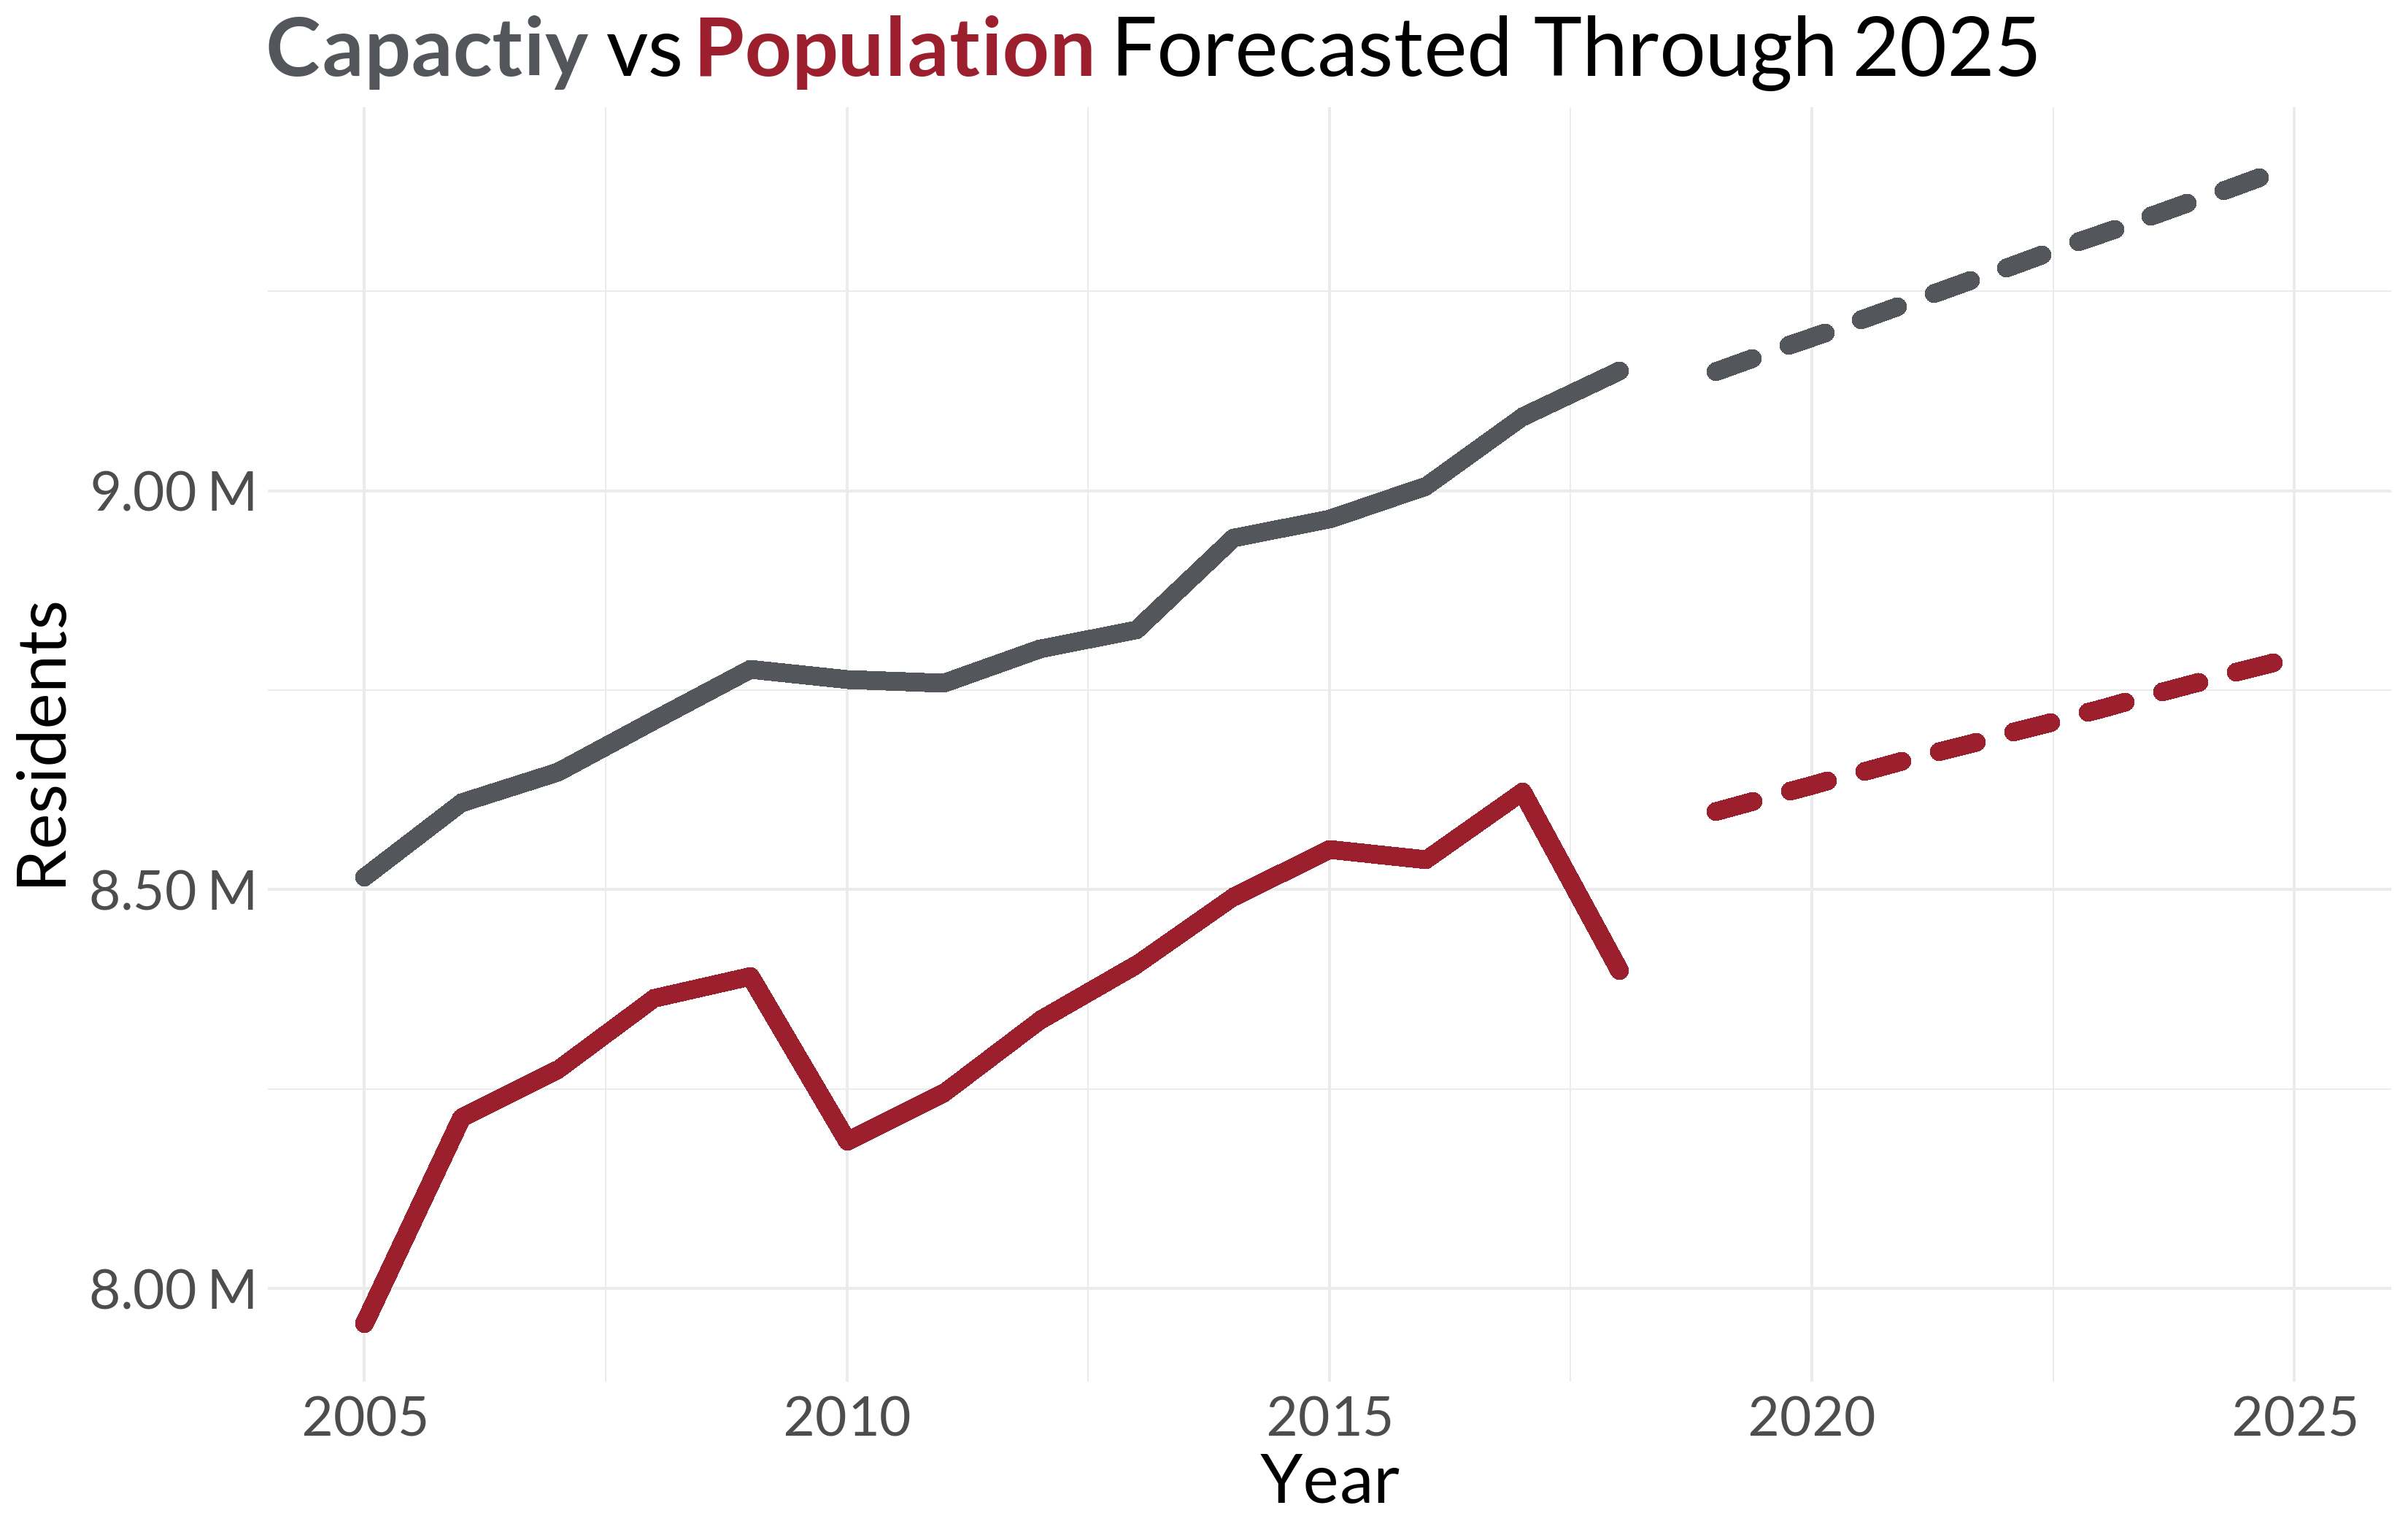
\includegraphics[height = 5.5in]{pics/pop_vs_capacity.png}
      \caption{Capacity and Population Forecast}
      \label{fig:my_label}
      \par}
  \end{figure}
  
  \end{block}


\newline\newline\newline

\end{column}

\separatorcolumn

\begin{column}{\colwidth}

  \begin{block}{COVID-19 Effects}
\begin{figure}[!tbp]
  
  \begin{multicols}{2}
  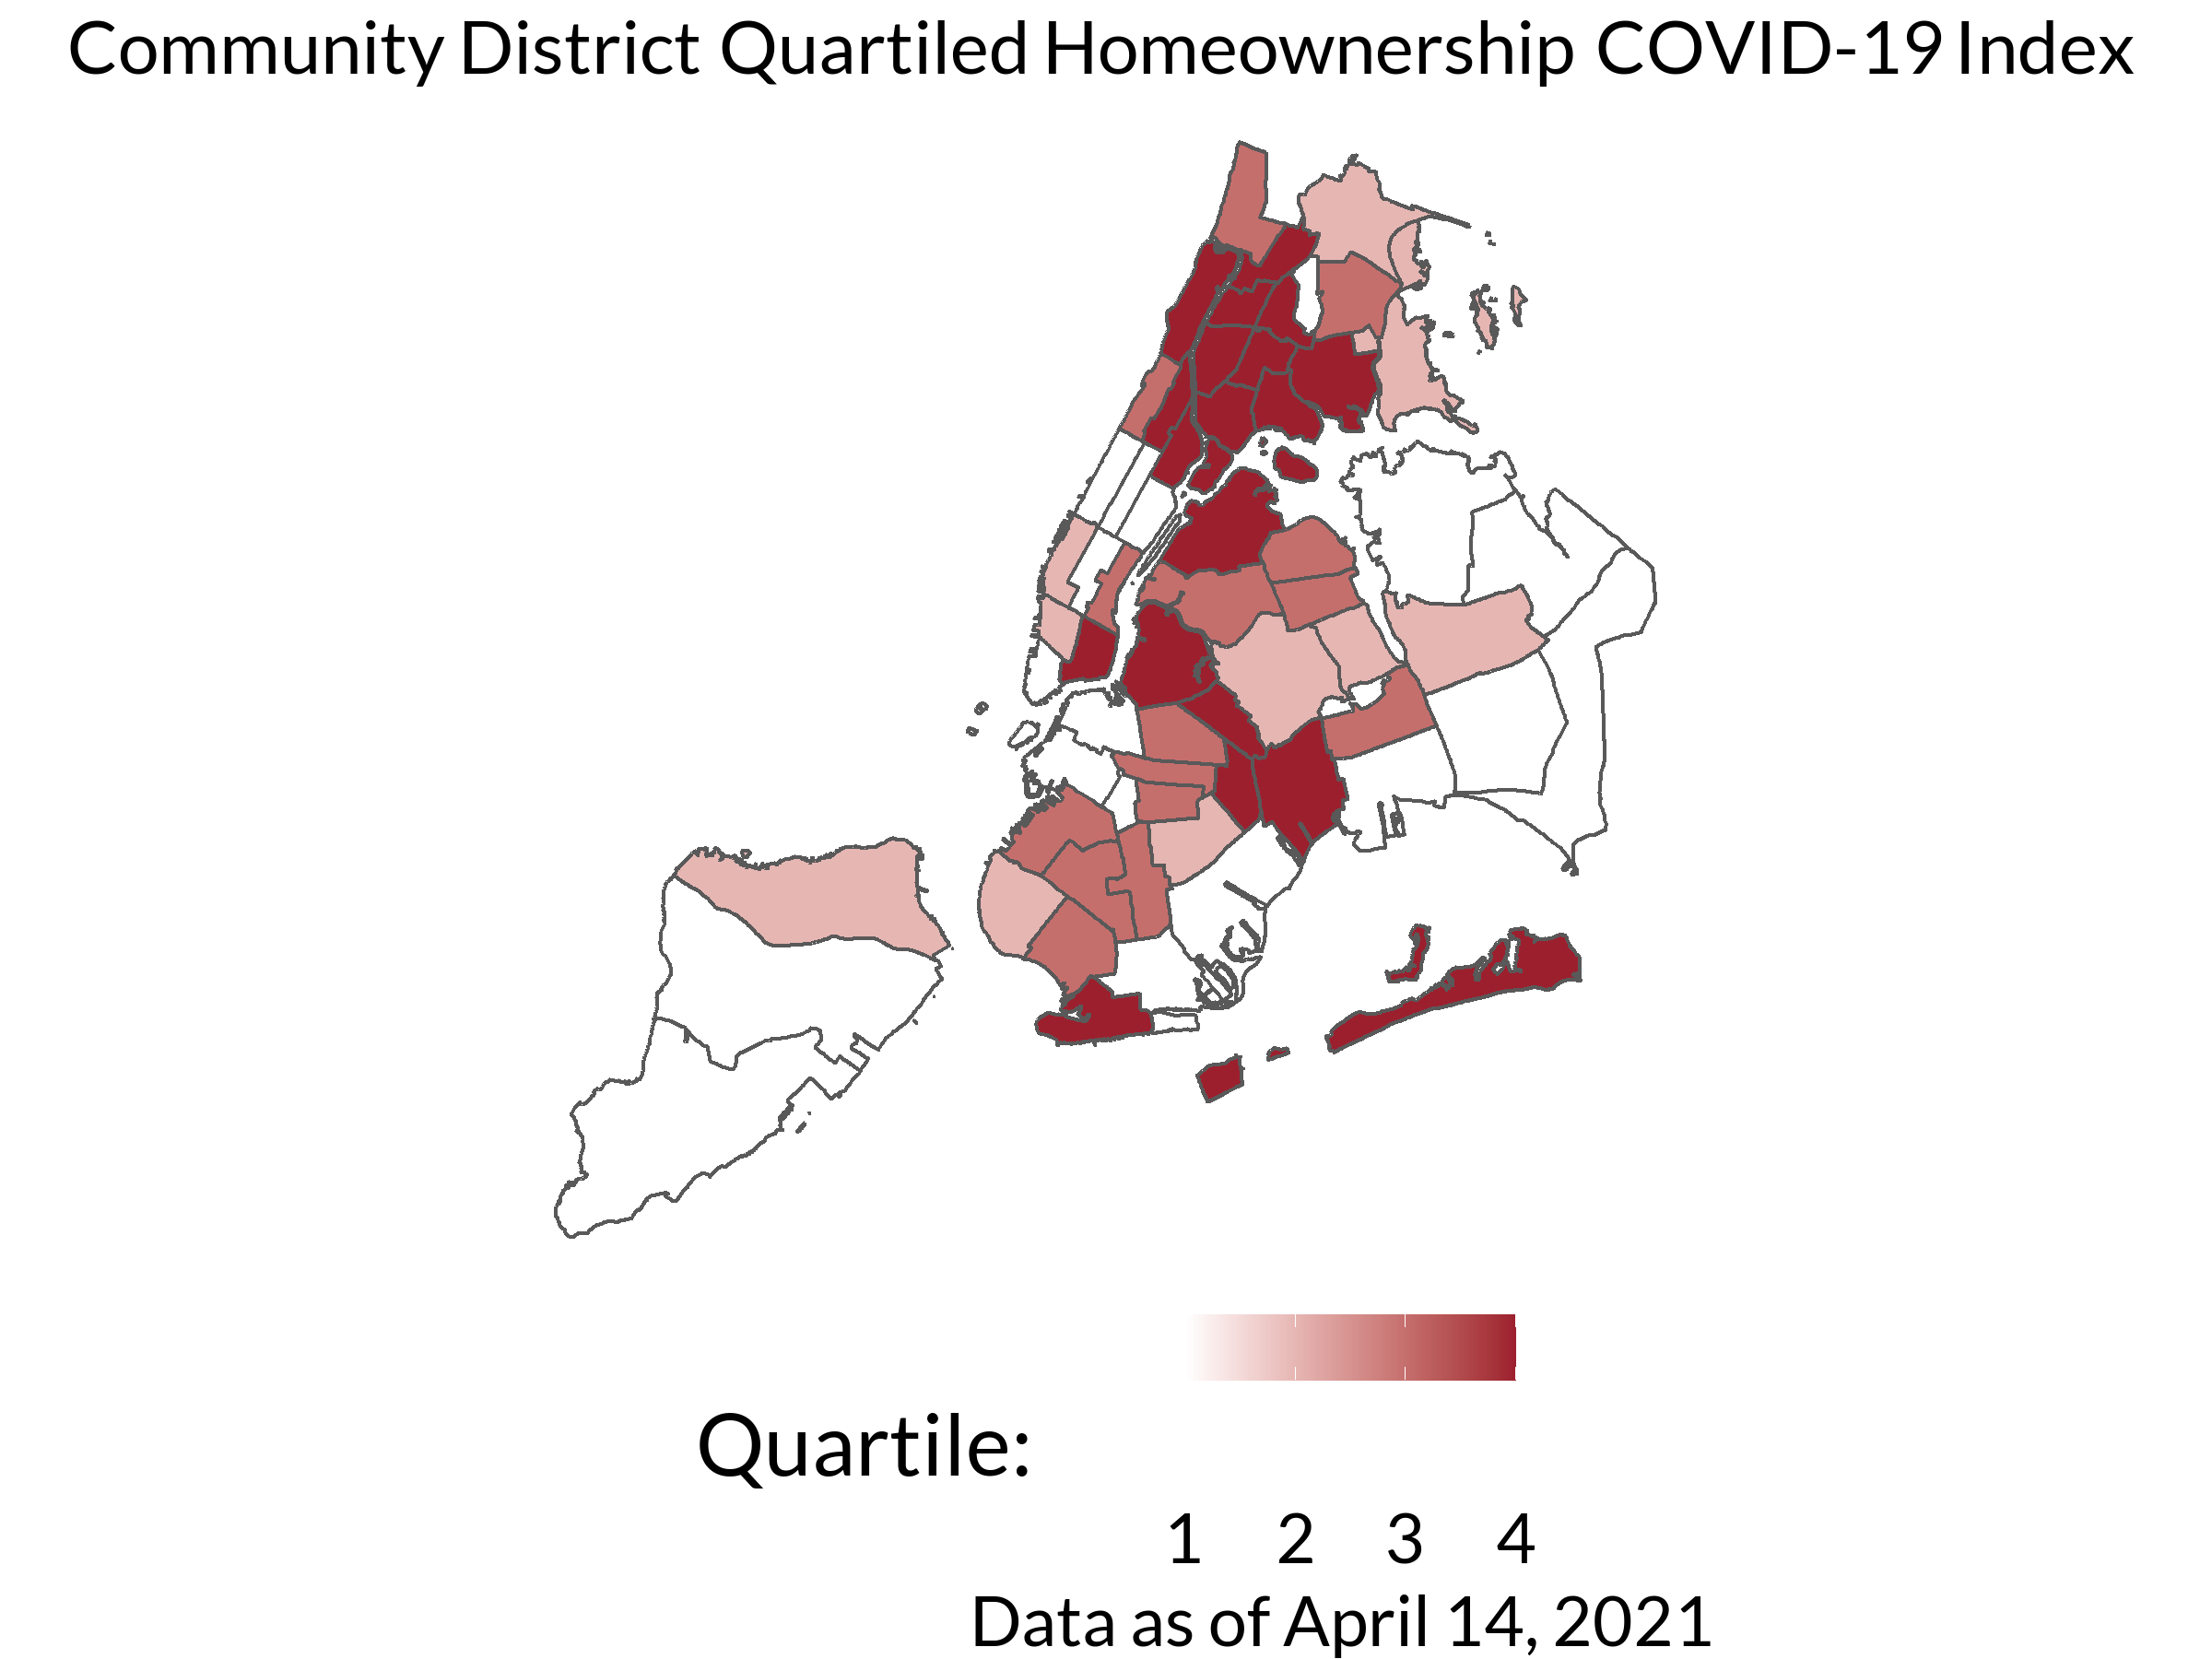
\includegraphics[width = 0.5\colwidth]{pics/covid_rate_4tile.png}
  \caption{COVID-19 Homeowner Index}
  \columnbreak
  \vfill\par
    This map shows an index of the effects of COVID-19 and Home Ownership Rate by community board. The index is calculated as $\frac{R_C}{R_H}$, or the district rate of infection over the home ownership rate.
    
    These variables are correlated at $R \approx 0.55$
  \end{multicols}
\end{figure}

\end{block}

\begin{block}{Identifying Community Boards}

    Using the data provided, as well as GIS data from NYC OpenData \textsuperscript{\cite{nyc}} and the Census \textsuperscript{\cite{census}}, demographic, housing, and infrastructure attributes were calculated at the Community District level. The below plots show the Community Districts identified for stimulus.
    

    \begin{figure}
        \begin{multicols}{2}
            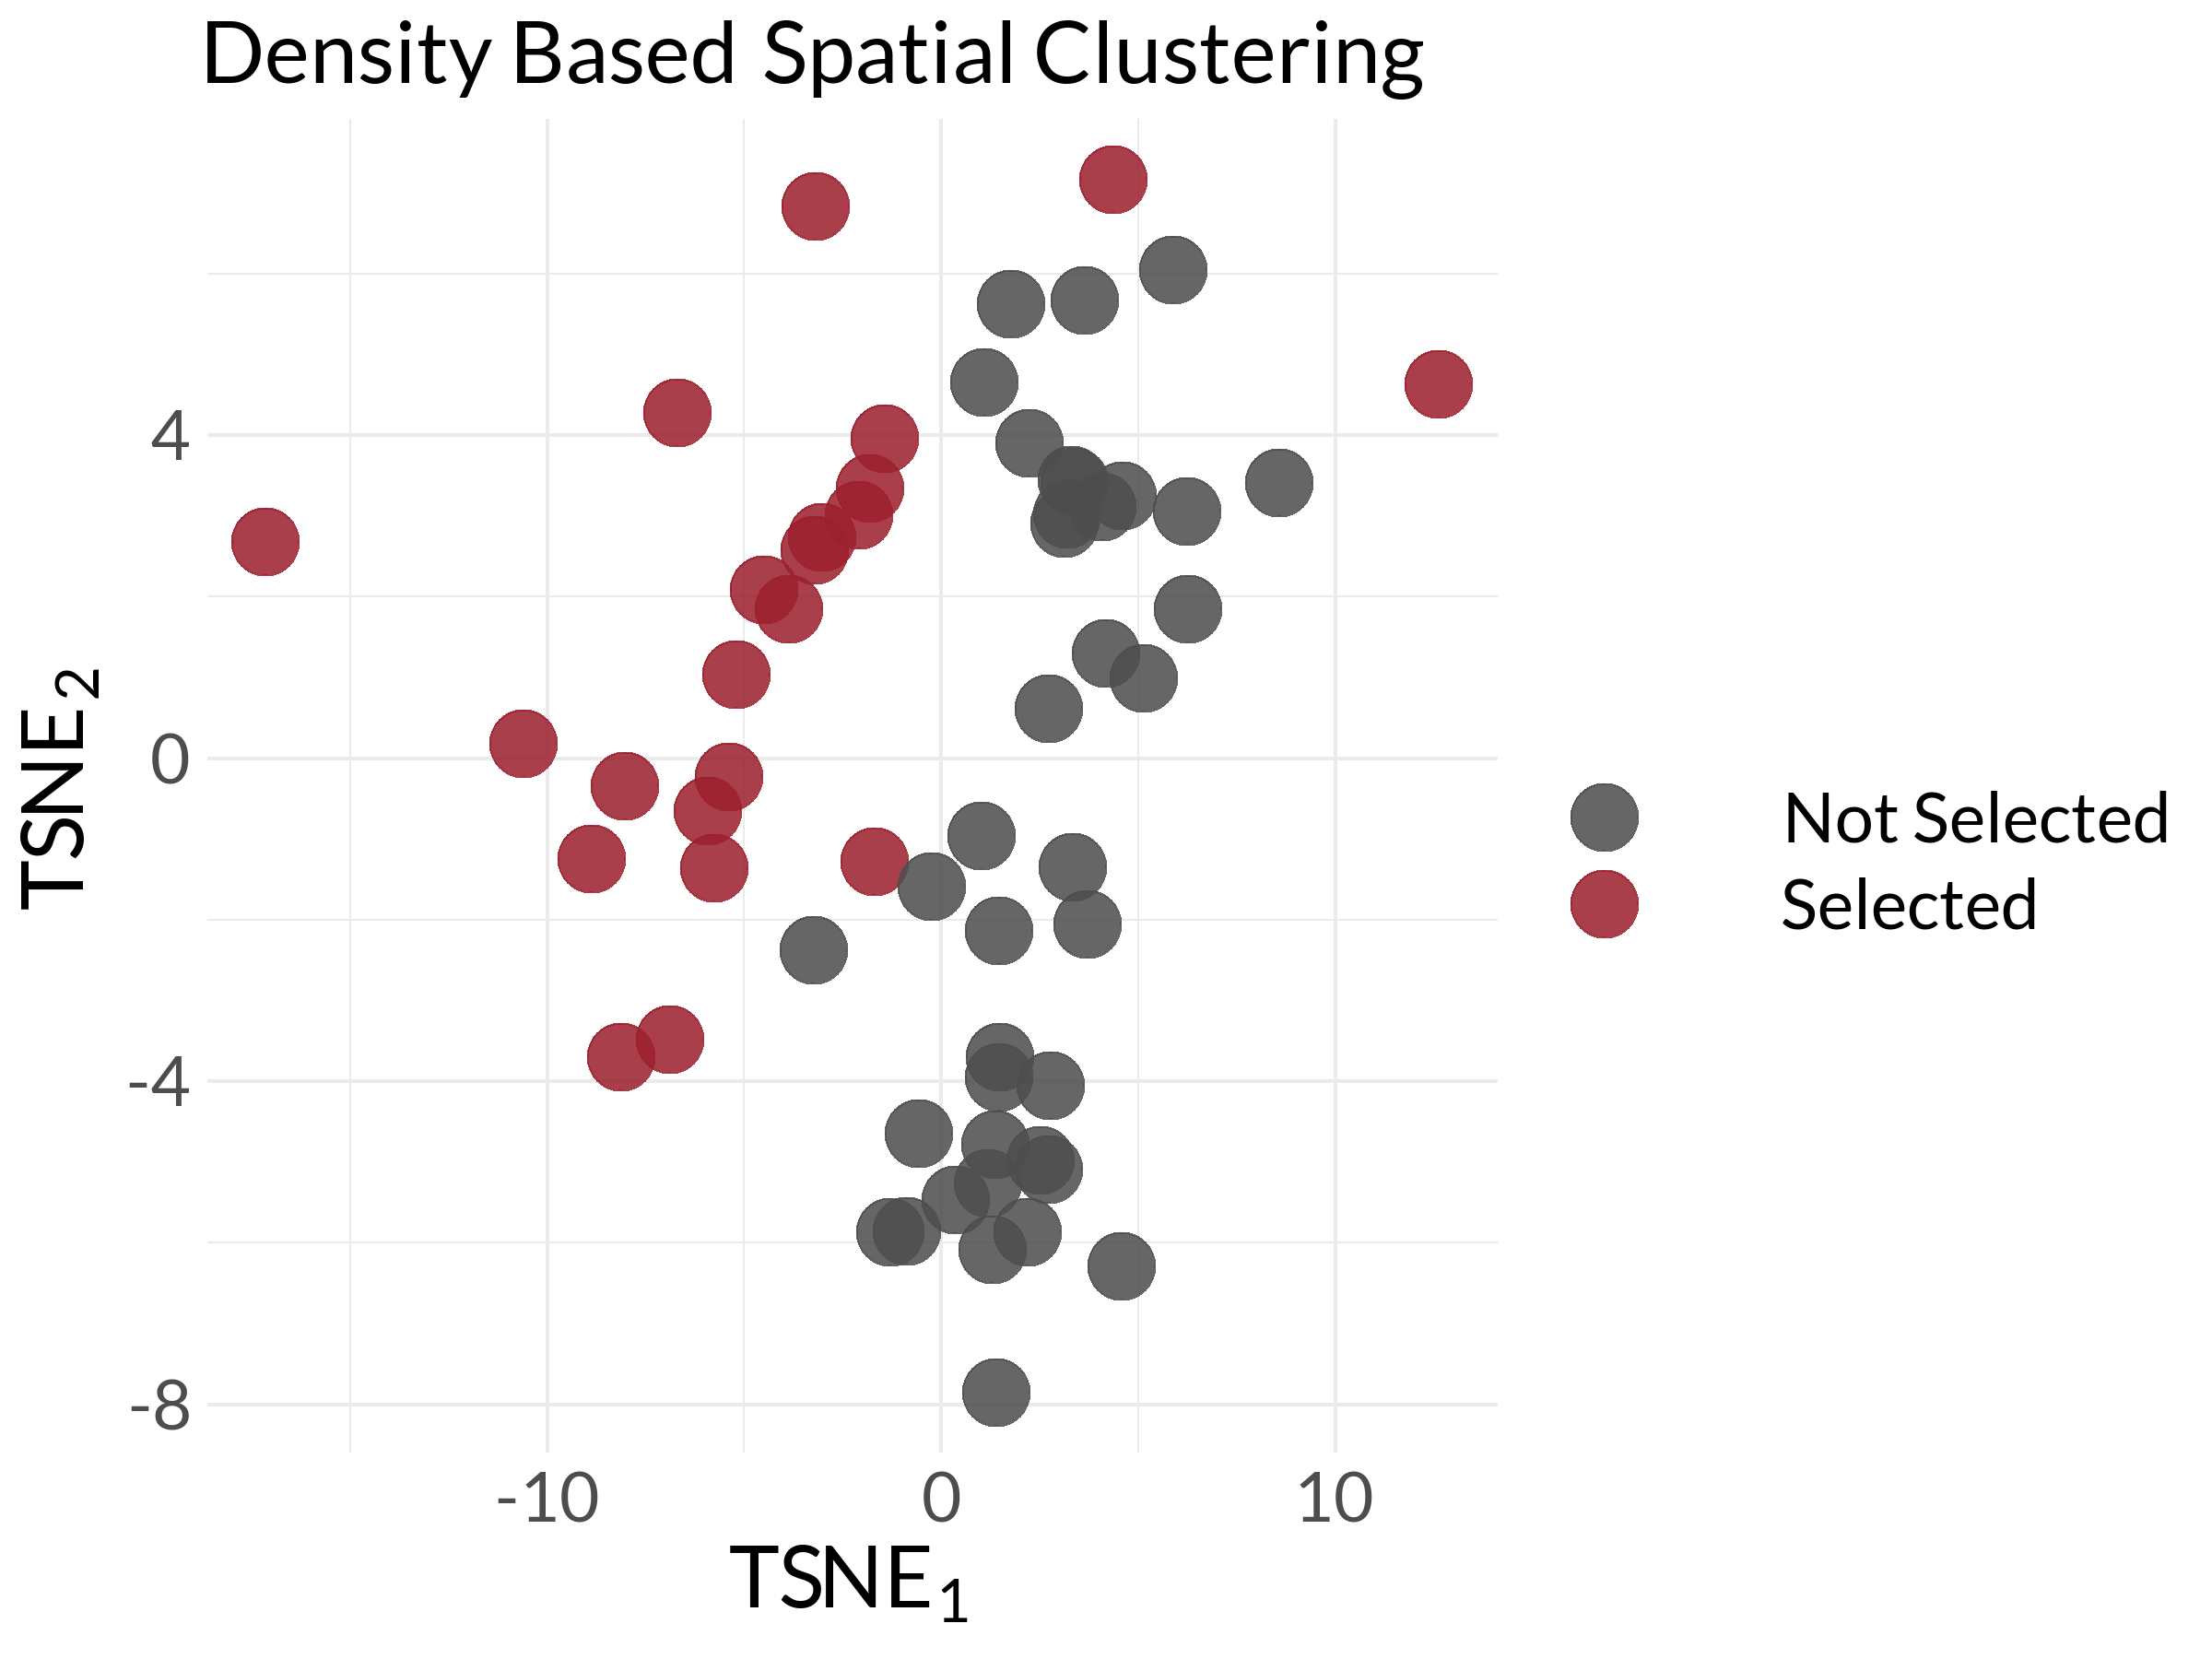
\includegraphics[width = 0.5\colwidth]{pics/dbscan_plot.png}
            \caption{TSNE and DBSCAN points}
        
             \columnbreak
        
            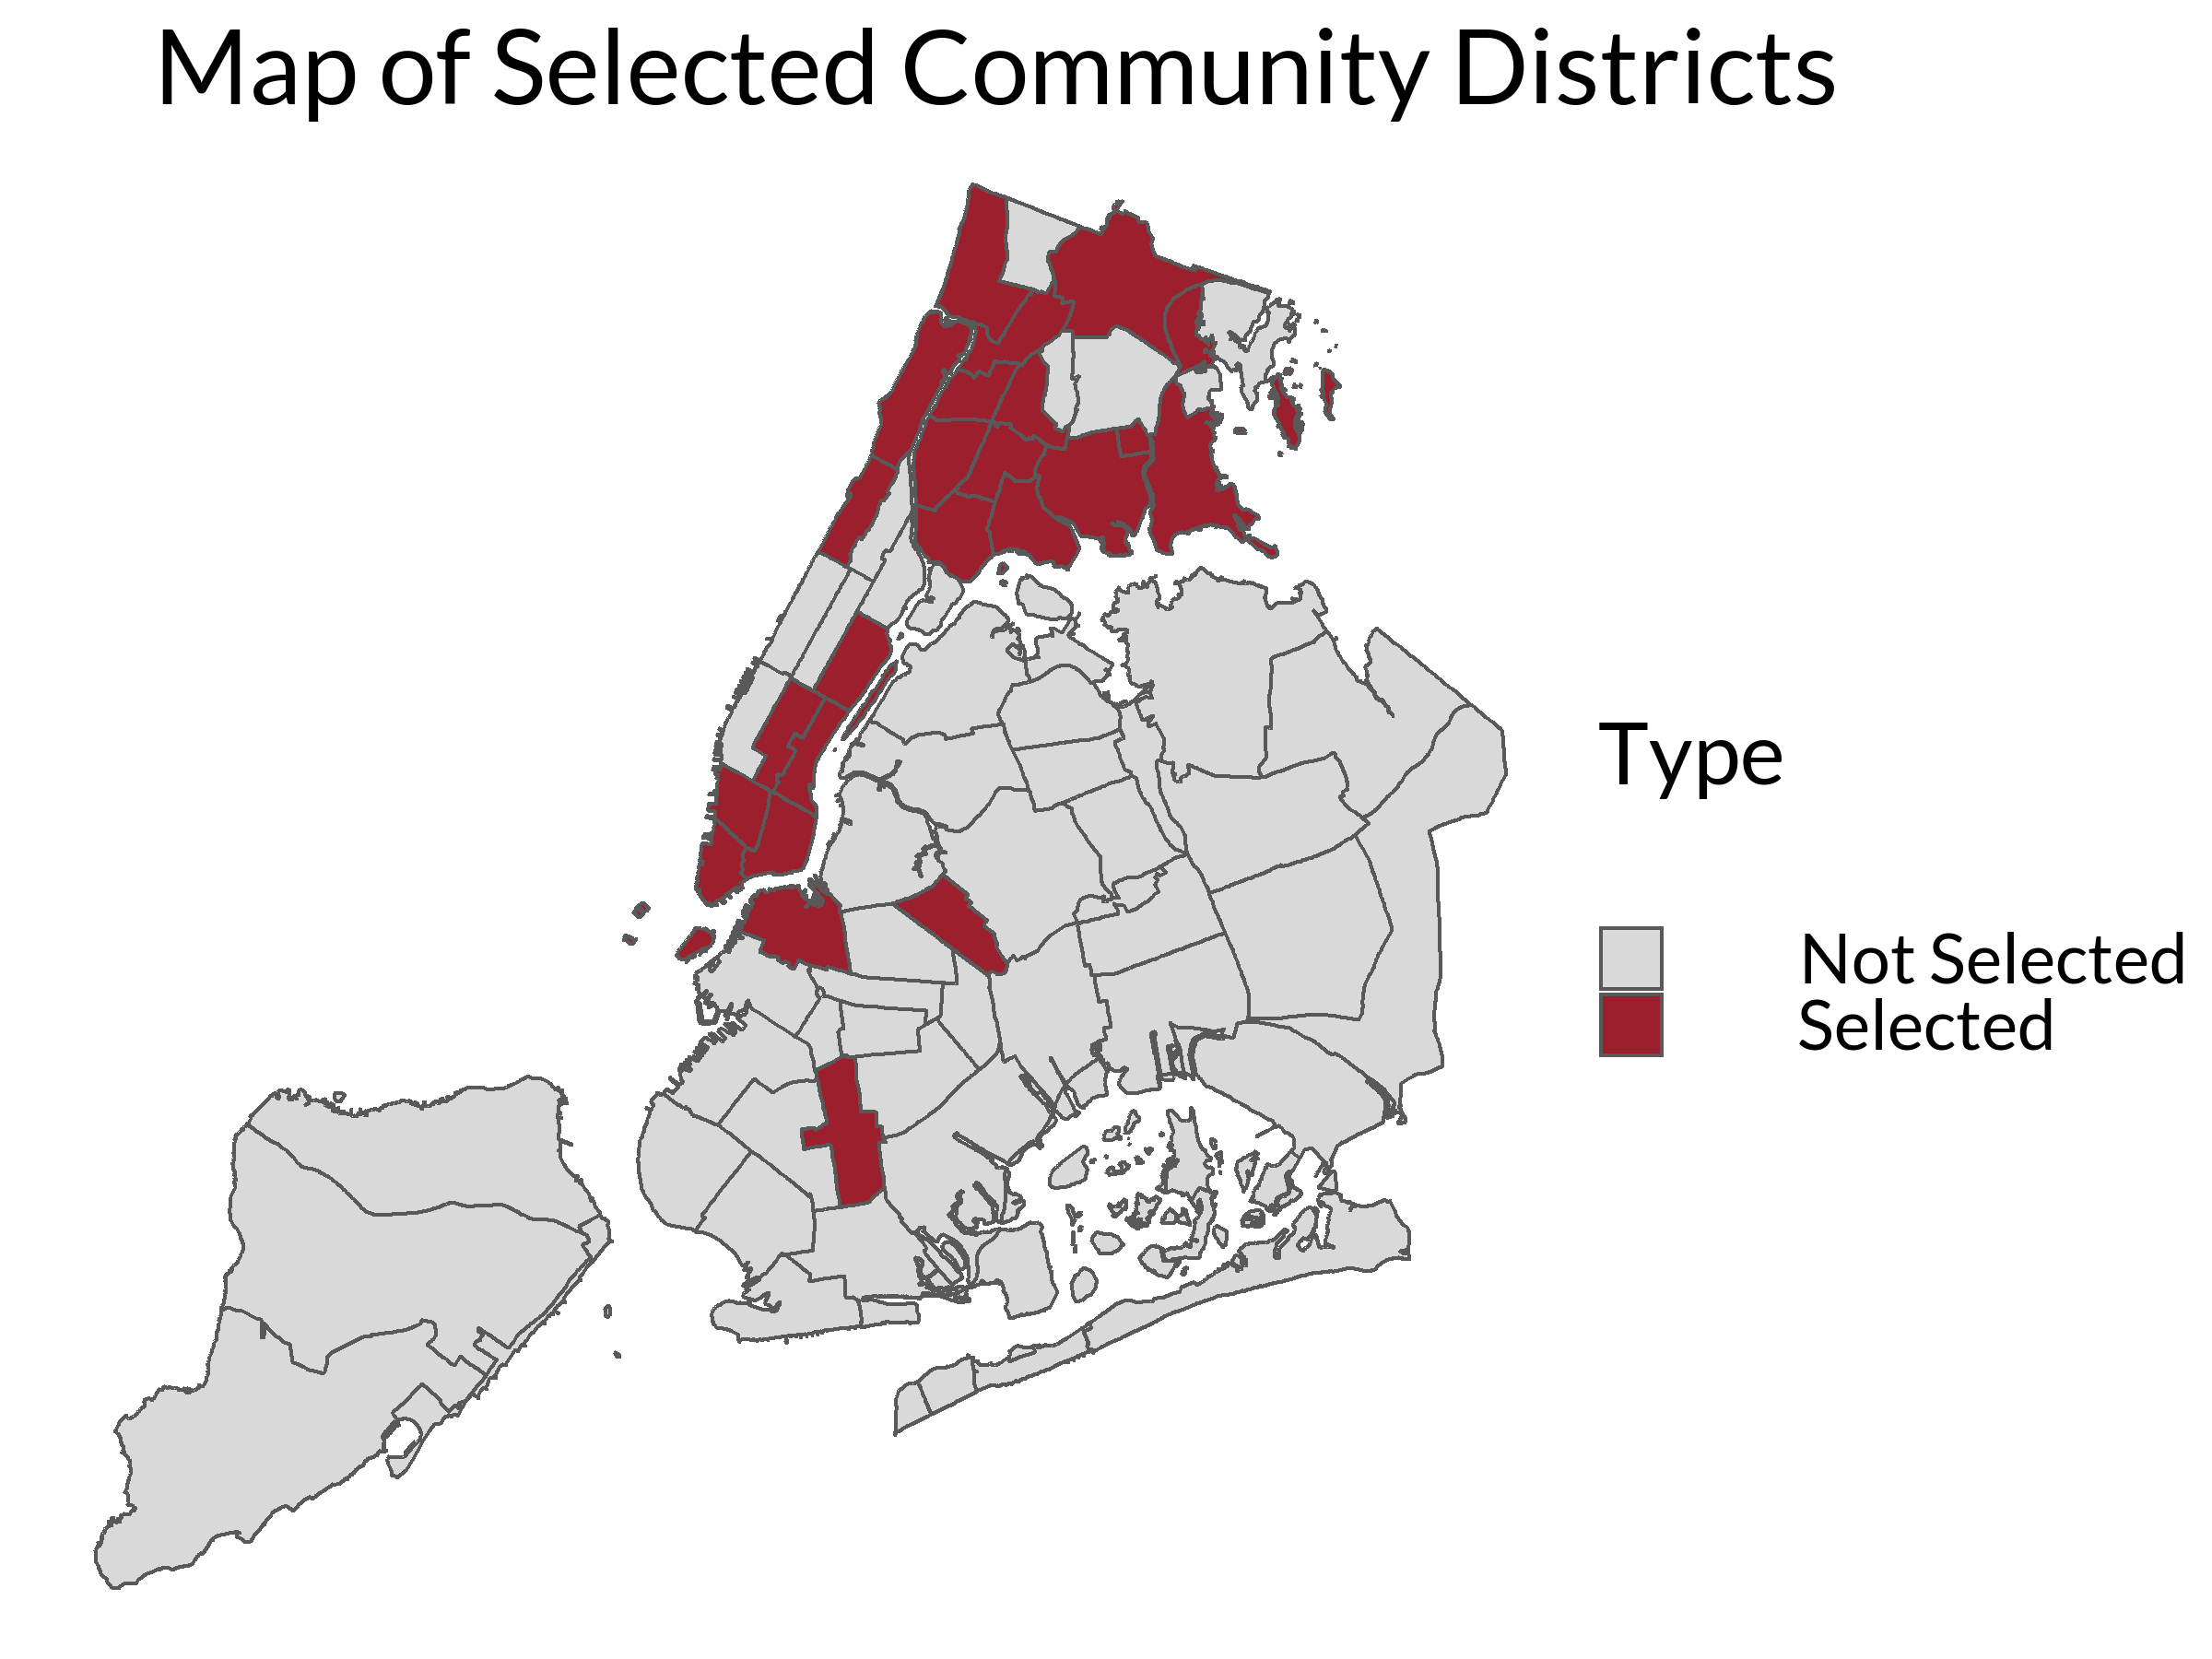
\includegraphics[width = 0.5\colwidth]{pics/dbscan_map.png}
            \caption{Selected Community Districts}
        
        \end{multicols}
    \end{figure}

  \end{block}

\begin{block}{Residential Area}


    \begin{figure}
        \centering
        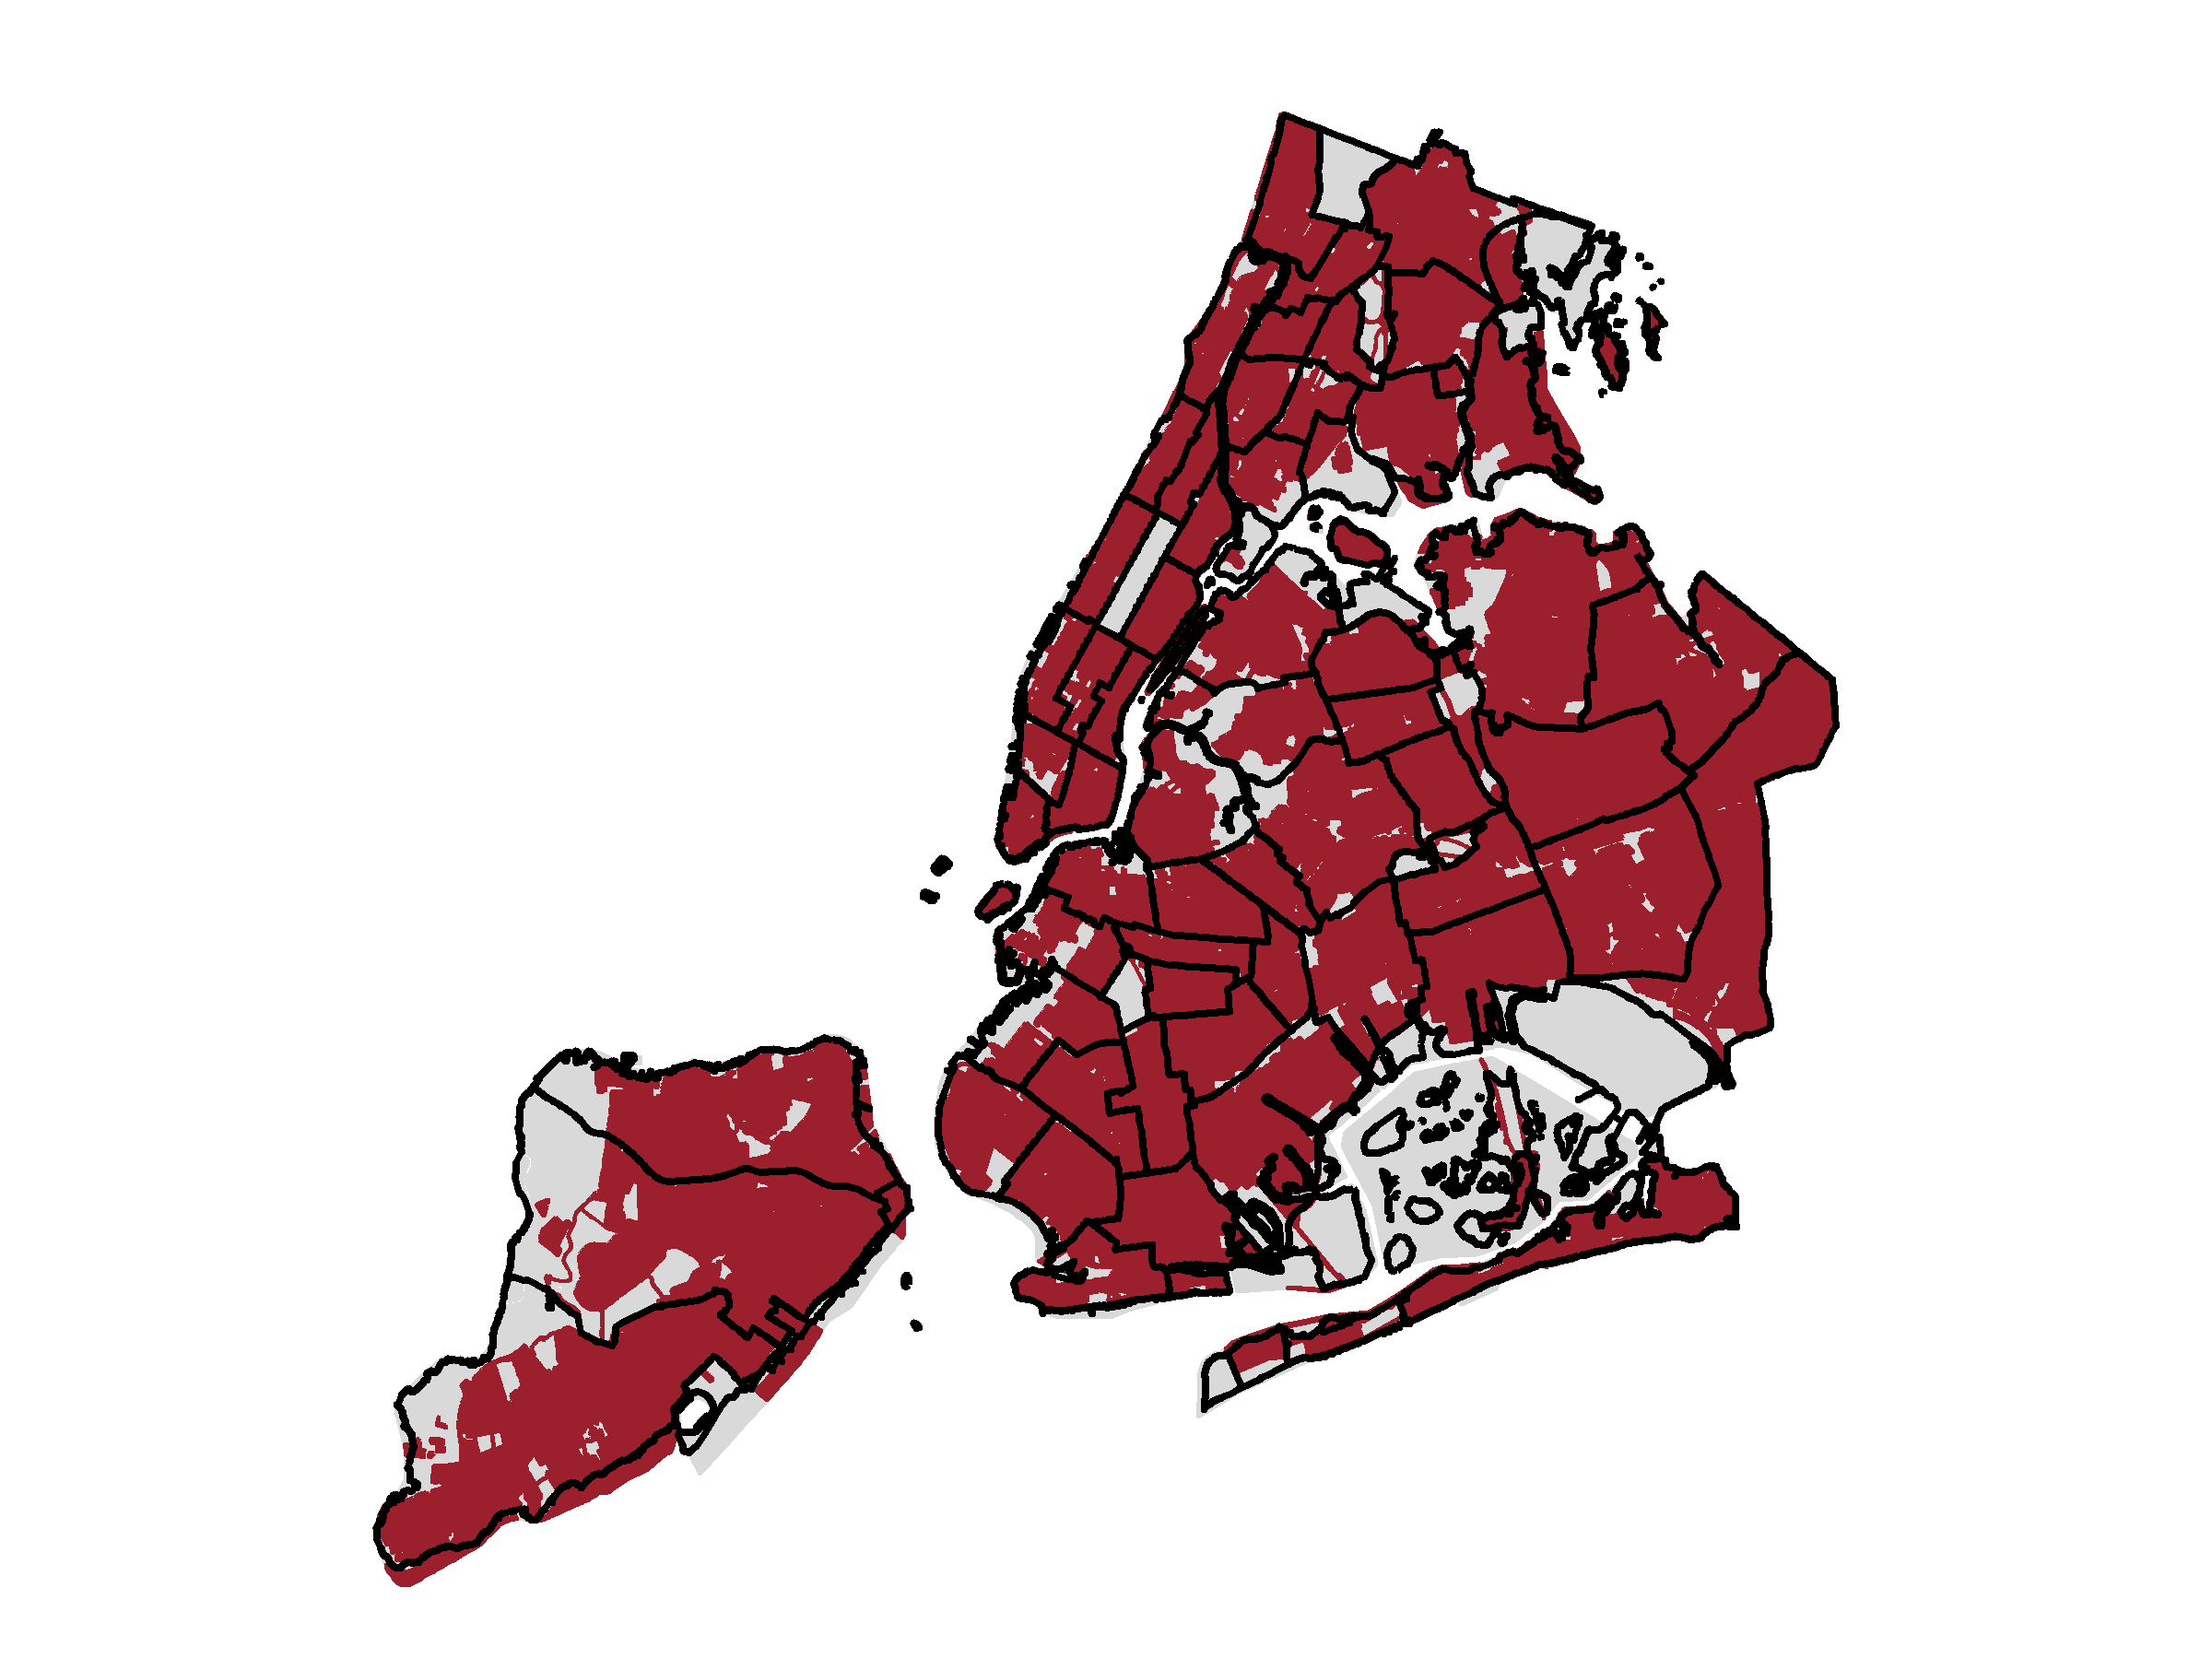
\includegraphics[height = 5in]{pics/zone_map.png}
        \caption{Residential Area by Community Board}
        \label{fig:my_label}
    \end{figure}
    
    \vspace{-1.5cm}
    
    The above map shows the land in New York City that is zoned for residential use by community board. In the community districts selected in Figure 3, this amounts to an average of more than 85\% of the overall district land, an increase of roughly 15\% from the NYC average.

\end{block}  
  
\end{column}

\separatorcolumn

\begin{column}{\colwidth}

  \begin{block}{Recommendation}

    At the current density of each selected community district, more than 73,000 housing units will be available per community district by 2025 when accounting for current construction plans. Factoring in the current density, total home ownership under this plan would account for more than 3.1 million New Yorkers.
    
    \begin{figure}
        \centering
        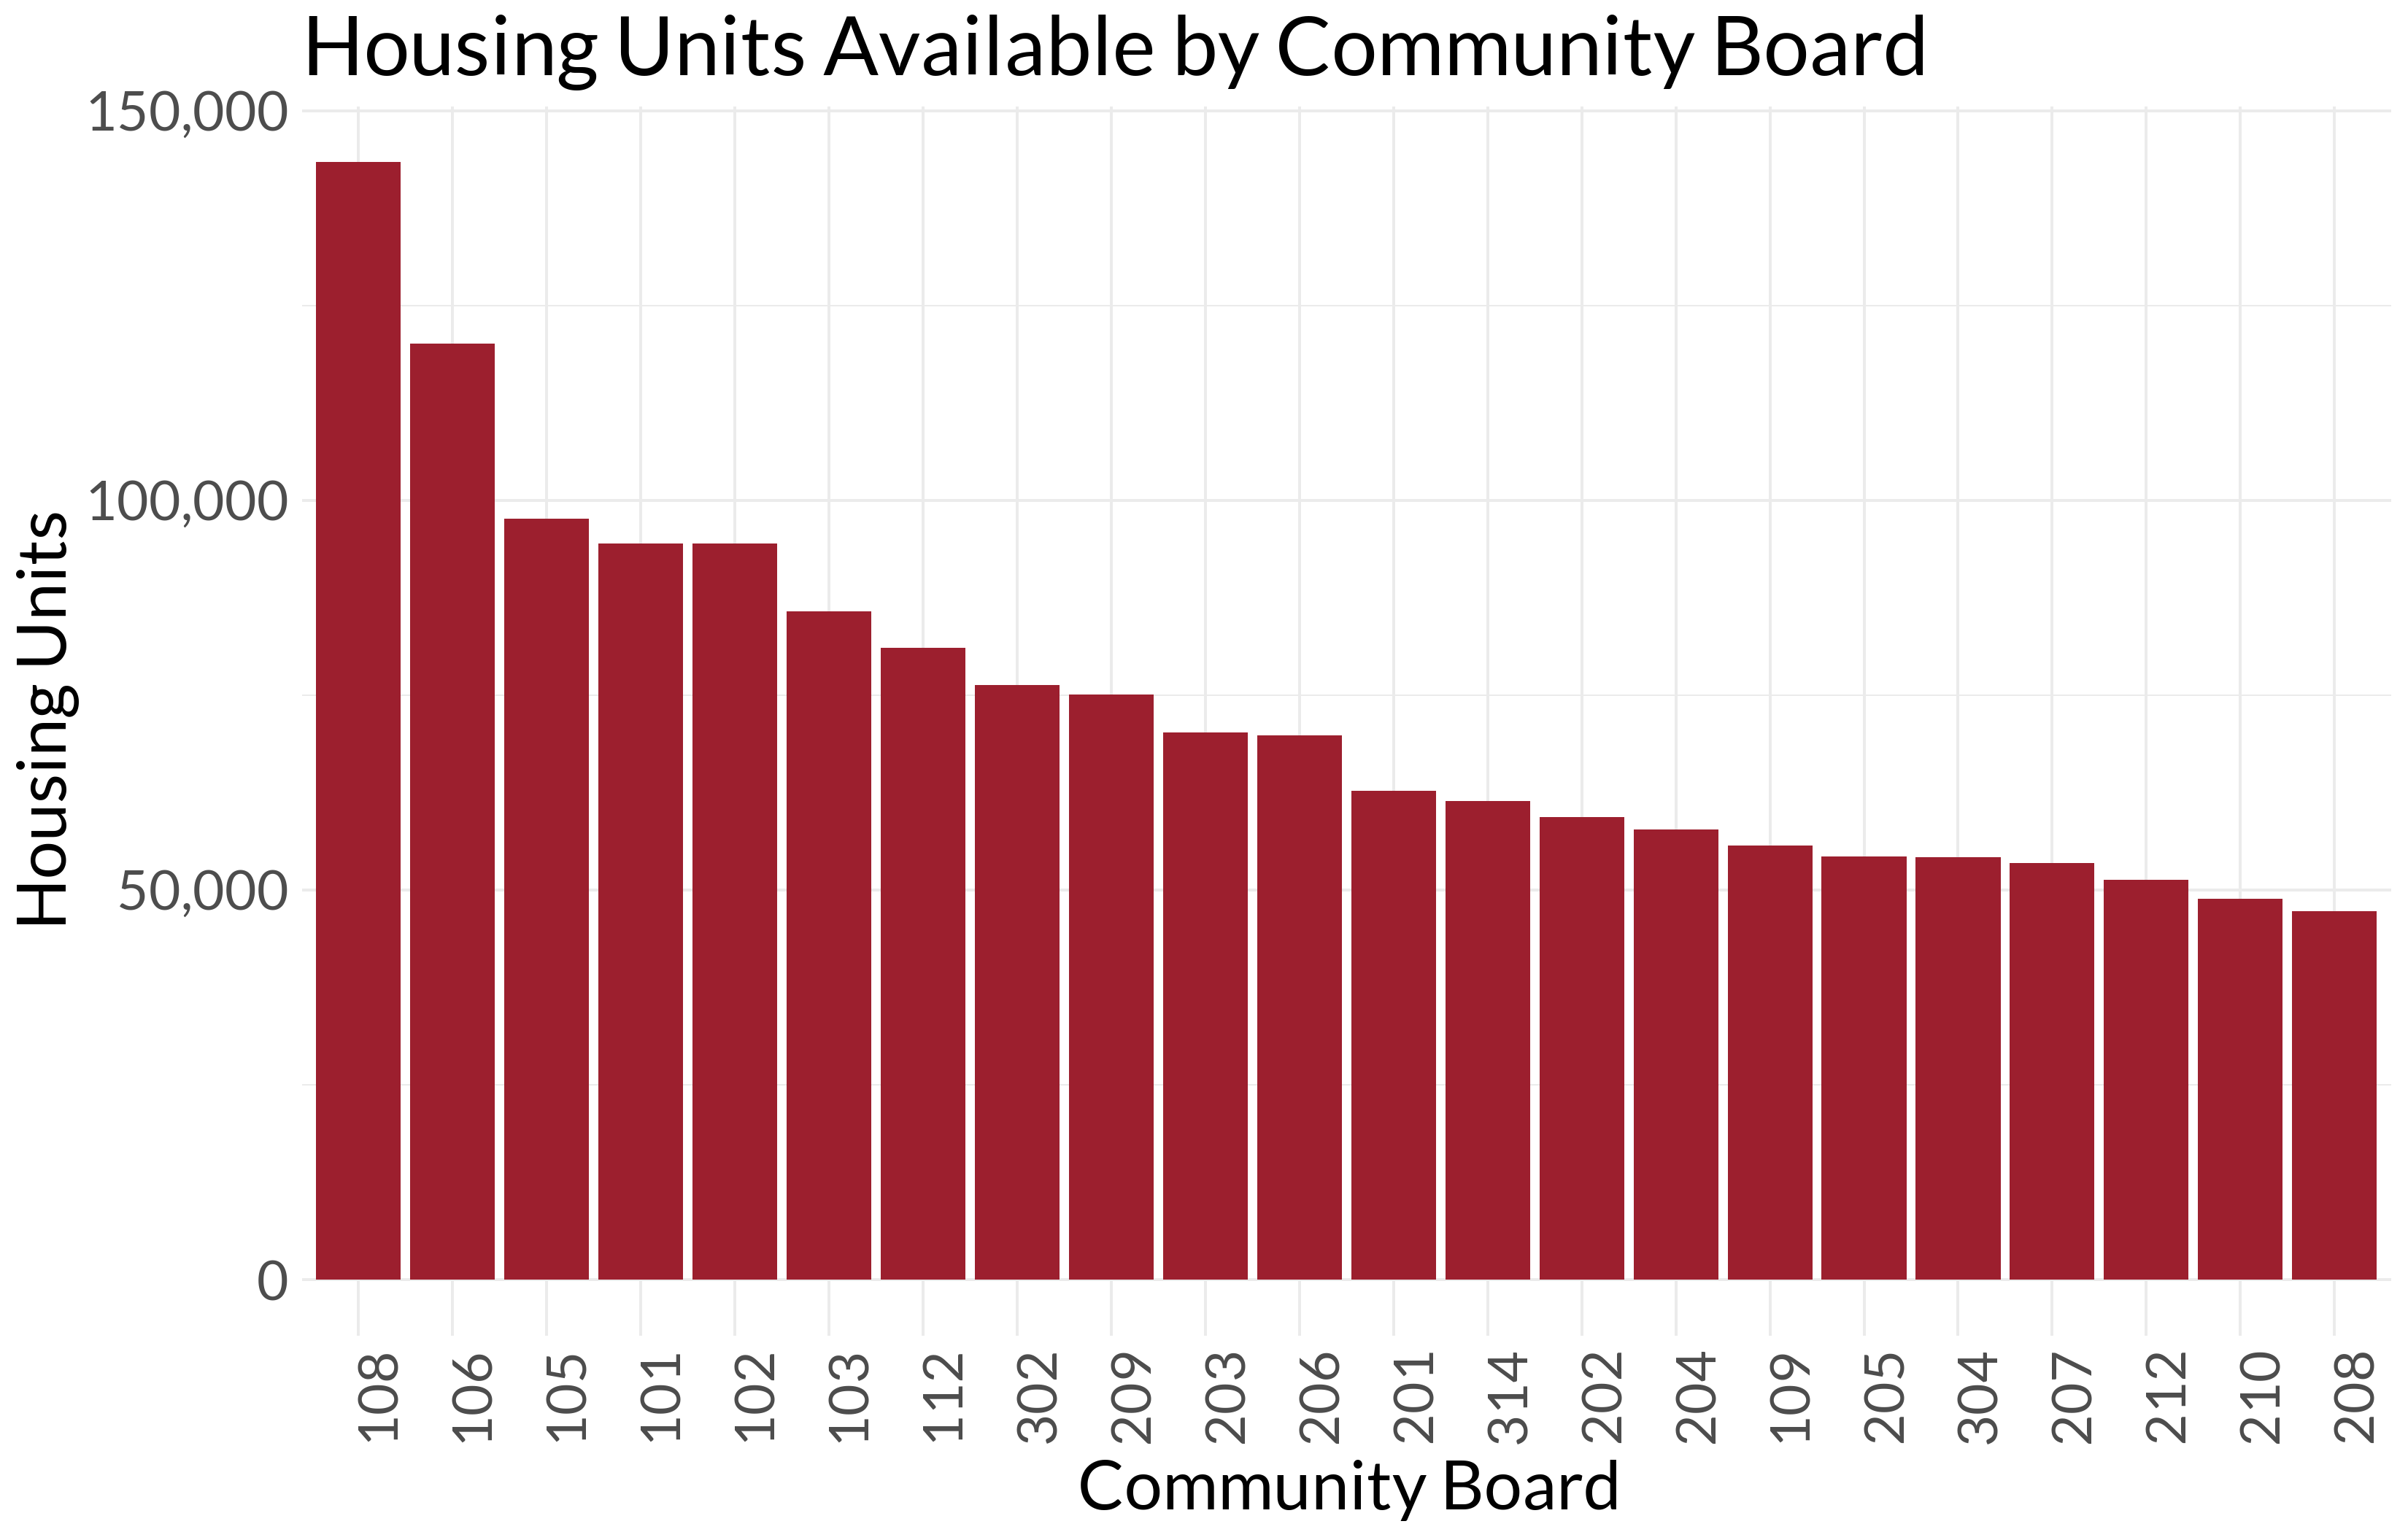
\includegraphics{pics/hunits.png}
        \caption{Housing Units}
        \label{fig:my_label}
    \end{figure}
    
    To make home ownership feasible in these districts, a multi-phase program could be implemented as below:
    
    \begin{itemize}
        \item \textbf{Renter Stimulus:} Current renters who purchase homes would qualify for a subsidy of their mortgage
        \item \textbf{Developer Credit:} Landlords who convert current rental units to homes for purchase would be subsidized for the cost
        \item \textbf{Landlord Tax:} Landlords who keep rental units past quota would be taxed proportionally to the number of units they own. 
    \end{itemize}

  \end{block}
  
  \begin{block}{Cost of Funding}
  
  \begin{itemize}
        \item \textbf{Renter Stimulus:} \$2.6 Billion: \$ 200/mo per affordable qualified mortgage
        \item \textbf{Developer Credit:} \$500 Million: \$5,000 credit per converted rental unit 
        \item \textbf{Landlord Tax:} +\$250 Million (est.): percentage of rent collected, rent stabilize units to avoid excise
    \end{itemize}
    
    For a total cost of \textbf{\$2.85 billion} per year or less than 70\% of the city's annual Affordable Housing Budget.
  
  \end{block}


  \begin{block}{References}

    \vspace{-1cm}

    \begin{multicols}{2}
    \nocite{*}
    \small{\bibliographystyle{plain}\bibliography{poster}}
    
    \end{multicols}

  \end{block}


  
\end{column}

\separatorcolumn
\end{columns}
\end{frame}

\end{document}
